% \documentclass[reprint,pra,twocolumn,superscriptaddress]{revtex4-2}
%[aps,prl,singlecolumn,superscriptaddress]
\documentclass[]{article}
\usepackage[english]{babel}
% \usepackage{ucs}
\usepackage[utf8x]{inputenc}
\usepackage{amsmath}
\usepackage{graphicx}
\usepackage{color}
\usepackage{biblatex}
\addbibresource{SiGe_ref_v1.bib}

\begin{document}
	
\title{Radio frequency reflectometry for qubit readout in silicon based quantum dot},
\author{Y.-Y. Liu, S. G. J. Philips, L. A. Orona, N. Samkharadze, A. Yacoby, L. M. K. Vandersypen}

\date{\today}


\begin{abstract}
	abstract to be written
\end{abstract}

\maketitle

\section{Intro} % (fold)
	\label{sec:intro}
	As Moore’s law begins to break down, new computational schemes will be necessary for improved computation performance.  Quantum computing is an exciting avenue that already boast algorithms that should provide speedups or perform tasks that are impossible on conventional computers\cite{bravyi2018quantum,farhi2018classification,carleo2017solving,shor1999polynomial}.  Of the physical platforms available, spin based quantum bits (qubits) in semiconductors are particularly promising \cite{vandersypen2017interfacing} \textcolor{red}{other good ref's that confirm this?}).  These qubits can be initialized quickly and with high fidelity through spin dependent tunneling to a neighboring Fermi sea.  Single qubit gates with fidelities above 99\% and two qubit gates above 90\% have been demonstrated.  The small size and localized nature of the control also lend themselves naturally to scaling to the number of qubits needed for a fully functioning quantum computer\textcolor{red}{ (we hope?)}. One particular interesting semiconductor material is silicon germanium (SiGe) which hosts a two dimentional electron gas (2DEG) where spin qubit can be formed. The qubits overlap with a small nuclear magnetic background compared to other materials, such as GaAs, which yields reduced spin decoherence due to the nuclear spin fluctuation\cite{hanson2007spins}. 

	Charge sensing is an important technique for measuring spin qubits because their long-lived spin states can be converted into detectable charge states.  This is usually done by Elzerman readout and Pauli-Spin blockade readout\cite{elzerman2004single,harvey2018high}. To detect a charge state, one can make use of a sensing quantum dot in close proximity ($d < \sim  300nm)$ to the qubit. The current through the sensing dot is strongly dependent on the charge state of the qubit due to the change of Coulomb potential.
	The easiest way (and most commonly used) way is to use measure the DC current through the sensing dot with a amplifier at room temperature (e.g. with a JFET). However, the sigal to noise is limited by the amplifier at 300K.
	In the same line of thinking, to reduce the noise temperature, people have also build DC amplifiers which work at base temperatures of dilution fridge, which has technique difficulty \textcolor{red}{Mark's paper?, dificulty is power budget at 10mK and also converting high impedace signal to a low one (?) will check with Raymond.}. It is thus of great interest to employ high frequency techniques that allows filtering low frequent noise and thus amplifying the signal with low background noise. %This is important because integration times are often the longest part of spin qubit experiments and reducing measurement time can therefore improve	qubit manipulation times significantly.
	
	Radio Frequency (RF) reflectometry has proven to be a very effective technique in gallium arsenide (GaAs) spin qubits and has enabled single shot readout with only several microseconds of integration \cite{Schoelkopf1998,fujita2017coherent} \textcolor{red}{more papers?}. However, silicon germanium (SiGe) has proved to be a more challenging platform in which to implement RF reflectometry due to larger capacitances to ground. Typical GaAs substrates are depletion mode while SiGe wafers are most often doped to be accumulation mode and require metallic electrostatic gates to cover all current paths so that the two dimensional electron gas (2DEG) can be populated \textcolor{red}{design papers?}. This capacitive coupling between the 2DEG and gates is undesirable for RF reflectometry because it provides low impedance leakage pathways to ground that are independent of the sensor dot (SD) that is capacitively coupled to the qubit and used to detect the qubit charge state\textcolor{red}{note that a ground reflects}. This reduces the sensitivity of the reflected signal to the qubit state. To solve that problem, the use of blocking resistor \cite{Volk2019} and  designing the accumulation gates \cite{Connors2020} has been reported to address this issue. %The capacitance to ground is also dependent on the gate voltage because the capacitance is zero when depleted and finite when accumulated which provides additional difficulty when designing the measurement circuitry.
	
	Here we demonstrate that RF reflectometry can be achieved in SiGe by utilizing the capacitance of the accumulation gates or  mitigating its effects with circuit board design.  There are two general approaches to reflectometry that differ in how the measured RF signal is carried to the lead of the sensor dot.  In the ohmic style, the signal enters the 2DEG through an ohmic contact so that it carried in the 2DEG itself all the way to the dot.  In the lead gate approach, it is carried by a gate which is capacitively coupled to the lead in the 2DEG near the sensor dot. For both scheme we have achieved sensitivity of the RF reflection to the resistance through the sensing dot and which enables us to perform charge readout of the target quantum dot. % We note that in both cases the sensitivity of the measurement is to the resistance through the sensing dot. and not the quantum capacitance because the signal always enters the SD from the lead and not directly from a gate.  
	%For both schemes careful care has been taken to reduce the effects of the capacitance on the sensitivity of tank circuit to the resistance of the SD and we discuss the different considerations that must be taken with each approach. 
	
%
%\color{gray} (original delft intro)
%
%The hard thing here is to convert the high impedance signal to a $50\Omega$ signal. This gives better results than room temperature amplification, but nowhere close the the theoretical noise limit.\\
%An alternate approach, which has been heavily used in GaAs quantum dot systems, is the use of what is called 'rf readout'. In this approach a RF signal is send to the sensing dot. Instead of current one now measures the reflection of signal at the sensing dot site. The reflection depends on the resistance of the sensing dot. Or formulated differently, a signal with an impedance $Z_0$ ($50\Omega$) is send down into the fridge. A matching circuit is build to convert $Z_0$ into $Z_1$ (e.g. $500k\Omega$). In other words, when the SD has a resistance of $500k\Omega$, all the signal is absorbed, where otherwise it will be (partially) reflected.\\
%
%In this work we will be focusing on charge sensing with a sensing dot. A difference in charge occupation is detected by a resistance change of the SD. In other words, this translates into a problems of accurately measuring a resistance (range $100k\Omega$ to $5M\Omega$). To tackle this problem there are a few ways of doing it.\\
%
%
%\color{black}

	

\section{RF Reflectometry circuit and theory} % (fold)
\label{sec:rf_reflectometry_circuit_and_theory}


\begin{figure*}[h!]
	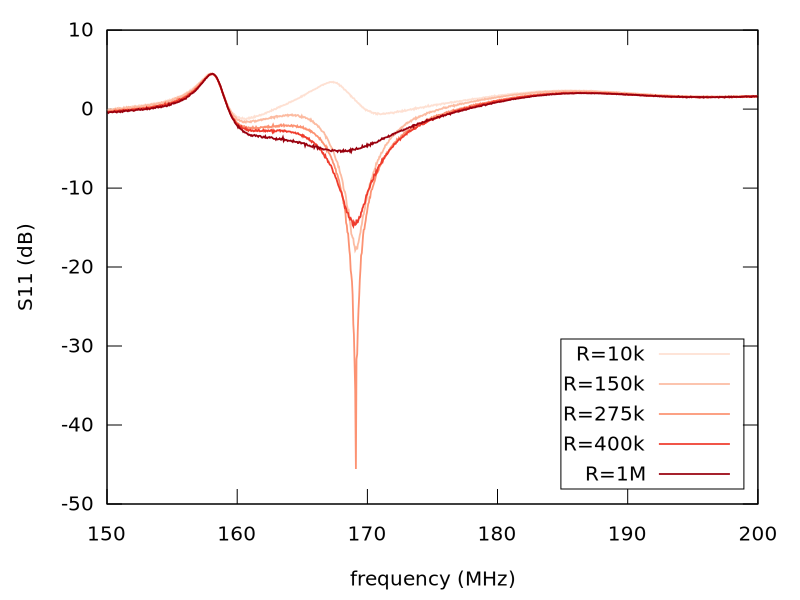
\includegraphics[width = \textwidth]{Illustrations/Overview/overview.eps}
	\caption{Circuit models for several device layouts with one sensing dot hooked up with RF readout on a mutilayer device type.  In the top image of each panel, a circuit model of the device is shown, in the bottom, a sketch of the physical device layout is shown. $L$ is the inductance of the inductor connected to the chip, $C_p$ is the parasitic capacitance of the inductor, the bondwire and the accumulation gate. In panel \textbf{(a)} a classical device layout is shown. In such a design the accumulation gate will have a large capacitance to the 2DEG below ($C_{2DEG}$). Panel \textbf{(b)} shows the circuit model and a schematic for the ohmic approach. In addition to the schematic in panel (a), a blocking resistor is added on the pcb to artificially reduce the effective capacitance of the accumulation gate. This resistor has as resistance $R_{block}$ and a capacitance $C_{block}$ (this capacitance is significant due to its macroscopic size). In panel \textbf{(c)}, the lead gate approach is shown, where the inductor is connected to the accumulation gate. This RF signal will couple in the 2DEG by the capacitive coupling of the accumulation gate. To make sure that the signal does not escape via the ohmic, a lead gate (see sketch) is added that allows to tune the resistance to the ohmic ($R_{Lead}$). In panel (d), an image is shown how the assembly of the inductor, resistor and lead gate looks like for the ohmic approach and a device image. Panel (e) shows a similar image for the lead gate approach.}
	\label{fig:overview}
\end{figure*}

%\subsection{Why SiGe is very different from the simples reflectometry} % (fold)
\label{sub:why_sige_is_very_different_from_the_simples_reflectometry}
In RF reflectometry, a fixed frequency signal is reflected off an impedance matching inductive capacitive (LC) tank circuit that is loaded with the sensing dot with resistance $R_S$, as shown in Fig.\ \ref{fig:overview}(a). The reflection coefficient of this tank circuit is given by $\Gamma=(Z-Z_0)/(Z+Z_0)$, where Z is the impedance of the loaded tank circuit and $Z_0 = 50 \Omega$ is the impedance of the RF cables of the system. When the device parasite capacitor $C_{\rm 2DEG}$ and contact resistance $R_{\rm 2DEG}$ can be ignored, the effective impedance seen by the reflectometry is $Z = i2\pi fL + 1/(1/(R_S + i2\pi fC_0)$ at an input frequency $f$. Here L is a lumped element inductor and $C_0$ represents the total capacitance of the circuit board, a lumped element capacitor and the parasitic capacitance of the bond wires to the device. 

$\Gamma$ is strongly modulated near $\Gamma = 0$, which occurs with the matching occurs as $Z=Z_0$ at a resonant frequency of $f=1/(2\pi \sqrt{LC_0})$ and a matching resistance $R_S=L/CZ_0$. $R_S$ of this sensing quantum dot is very sensitive to the electric potential of its environment, and thus to the charge states in the nearby dots. Combining the rf sensitivity to the load impedance $Z\sim Z_0$ and the sensitivity of $R_S$ to the environment, the tank circuit is designed with L and C0 chosen to yield $Z_{\rm match} = L/CR_s= 50 \Omega$  for the most typical $R_S$ of a single quantum dot, ranging from 50 -- 400 $k\Omega$
% \footnote{\color{blue} is this correct for SiGe, we usually are somewhere in between 400k and 1M? (both Wisconsin en Delft devices)} LYY: let's discuss on this? we ususally can achieve 50 to 300 kOhm, otherwise the signal would be very small
.   For GaAs, this simple model is sufficient to capture the observed behavior. 

In SiGe, the simple tank circuit model fails because $R_{\rm 2DEG}$ and $C_{\rm 2DEG}$ is no longer negligible.	Fig.\ \ref{fig:overview}(e) demonstrates a typical overlap style device.  A quadruple quantum dot is formed with the lower set of gates and two sensors are formed with upper gates. Large accumulation gates control the leads from the ohmics to the quadruple and sensor dot’s (in GaAs one has depletion mode devices.)
Extra parasitic capacitance is added by the accumulation gate (large gate on top of the 2DEG, see figure\ \ref{fig:overview}(a)) which has a typical value of \color{red} 0.1 -- 1 pF \color{black} in total. This capacitor couples to ground through the line resistance $R_{\rm block}$ and capacitor $C_{\rm ground}$ to the environment. RF signal will then pass a lossy 2DEG channel with resistance $R_{\rm 2DEG}$ and then shunts to ground. This significant $R_{\rm 2DEG}$ and $C_{\rm 2DEG}$ reduces sensitivity of $\Gamma$ to the sensor dot $R_S$. %Careful analysis into the role of the parasitic capacitance is necessary to understand and mitigate its effects. This analysis also guides the modification in device designs for acceptable $C_{\rm gate}$ and $R_1$.	


To circumvent this problem, we propose the following approaches:
\begin{itemize}
	\item Adding additional components on the PCB to compensate for large parasitics (fig 1\textbf{b}), which we call it Ohmic approach.
	%\item Reduction of capacitance of the accumulation by moving the ohmics close and breaking the 2DEG (fig 1\textbf{c}).
	\item Use the large capacitance of the accumulation gate to your advantage, use a lead gate for the ohmic (fig 1\textbf{d}), which we call it lead gate approach.
\end{itemize}



\subsection{Ohmic approach circuit and model} % (fold)
% \footnote{\color{blue}lumped element on pcb not introduced.}


\begin{figure*}[h]
	\includegraphics[width = \textwidth]{Illustrations/HarvardFigure2_v5.pdf}		
	\caption{(a) and (b) Resonant frequency and impedance matching condition as a function of $C_0$ and L with fixed parameters of $C^*_{\rm gate} =$ 0.2 pF and $R_{\rm cont}$ = 3 kOhm. The simulation is achieved by solving for the conditions that give the loaded tank circuit an impedance of 50 Ohms. We note unplotted areas cannot achieve matching with 50 Ohms with a physical solution ($f>0$, $R_S>0$). The blue (red) dot represents the parameters we used before (later) in the experiment. 
		(c) Impedance matching condition as a function of R1 and L with fixed $C^*_{\rm gate}$ = 0.2 pF, and $C_0$ = 1.6 pF. The red dot represents the parameters used in panel (a-b). 
		(d) The calculated matching condition as a function of inductor L and  $C^*_{\rm gate}$ with C0 = .76 pF, and $R_{\rm cont}$ = 3 kOhm. }
	\label{fig:HarvardTheory}
\end{figure*}



	\label{sub:ohmic_approach_circuit_and_model}
	
	The ohmic approach is a direct implementation of RF reflectometry as it was performed in GaAs.  As mentioned, the significant resistance of the 2DEG and capacitance to the accumulation gate prevent using the simply RLC model used in SiGe.  Instead, the device is a continuous series of capacitors and resistros, as shown in Fig. 1(a).  For simulation simplicity, this can be treated as a single resistance, $R_{\rm cont}$ and single capacitance, $C_{\rm gate}$.
	
	
	As the simplest solution, We first investigate the possibility of PCB board improvement in order to achieve rf-reflectomery, using the same model in Fig.\ \ref{fig:overview}(b). We note that this is the same model for GaAs and SiGe and the main difference is how much the parasite capacitor $C_{\rm gate}$ will play a role. While it is hard to reduce $C_{\rm gate}$, we can reduce its impact by increasing C0 on board. However, increasing $C_0$ potentially reduces the 50 Ohms matching impedance $R_s=L/(C_0Z_0)$. To keep the impedance matching happens at a realistic $R_S$ for a single dot, the increased $C_0$ is compensated by the onboard inductor $L$.
	
	We initialed the tank circuit with an inductator of 760 nH on board and parasite capacitor $C_0$ from the device and board, which works for GaAs. With a SiGe device, however, we measured a resonance frequency $f=220$ MHz before the accumulation gates populate the 2DEG, and $f = 180$ MHz after we accumulate the lead. $\Gamma$ is only dependent on the lead gate and is not sensitive to $R_s$. From the two resonance frequencies, we estimate a constant $C_{\rm gate} =$  0.45 pF and $C_0=$ 0.8 pF. The ratio $C_{\rm gate}/C_0$ is above 50\% and cannot be ignored. 
	
	In order to minimize the leakage of RF signal through the gate to ground, we place resistors between the gate wire bonds and the RC filters that are used for the DC lines. This improvement is limited by the remaining parallel pathway to ground with $C_{\rm ground}$. With sufficient $R_{\rm block} > 10$ kOhm, the total leak to ground can be simplified into an effective capacitor $C^*_{\rm gate} = 1/(1/{C_{\rm gate}}+1/C_{\rm ground})$ which we have found to still be around 0.2 pF from the resonance frequency. This modifies the circuit model, as shown in Fig.\ \ref{fig:overview}(b) so that there is a capacitive pathway straight to ground that is independent of the SD.   
	
	We now explore the parameters range of the on-board elements where we can achieve matching. In Fig.\ \ref{fig:HarvardTheory} (a-b) we examine the matching frequency and sensor resistance respectively as functions of L and $C_0$ with fixed $C^*_{\rm gate}$ = 0.2 pF, and a contact resistance $R_{\rm cont}$ = 3 kOhm.  The most important aspect of this figure is that there are large parameter regimes in which best matching cannot be achieved, shown in white.  We see that the parameters used as for GaAs lie deep within this region (marked as blue). It is unsurprising that the tank circuit is very insensitive to the sensor resistance in this regime. The parameters marked as the red dot in is far from the boundary between the matching and non-matching regions. 
	We find that the dependence of the frequency and matching resistance behave as they would for the naïve tank circuit model with modified parameter $C^*_0 = C_0 + C^*_{\rm gate}$ and $R^{\rm match}_S = Z_{\rm match}-R_{\rm cont}$. Near the boundary, we find the best matching impedance can change by a factor of 10 $\sim$ 100 with only 1\% change in $C_0$ or $L$, and thus is not ideal as this is the typical variation between samples. This simulation provides a regime in which the frequency and matching resistance can be tuned by selecting the proper values of $C_0$ and L for an existing device design.   
	
	We note that $R_{\rm cont}$ is hard to extract from direct measurement so the above simulation is based on a very rough estimation on this value. We further explore the impact of $R_{\rm cont}$ to validate the above estimation. Figure\ \ref{fig:HarvardTheory}(c) plots $R^{\rm match}_S$ as a function of inductance and $R_{\rm cont}$ when $C_0 = 1.6$ pF and $C^*_{\rm gate} =$ 0.2 pF. When $R_{\rm cont}$ = 0 then the model still can be simplified as a standard tank circuit with $C^*_0 = C_0 + C^*_{\rm gate}$. 
	With a larger $R_{\rm cont}$ there are two possible regimes, which are split by $L$. For small inductance $L<1200$ nH, there matching conduction $R^{\rm match}_S$ decrease with $R_{\rm cont}$. This is expected as simple model estimated  $R_S = Z_{\rm match}-R_{\rm cont}$ would be best matched. However, the  $R^{\rm match}_S\sim 10$ kOhm is too conductive for a quantum dot. For large inductance $L>1200$ nH,  $R^{\rm match}_S$ increases with $R_{\rm cont}$ until it diverged on the boundary. It is thus necessary to keep $R_{\rm cont}<4$ kOhm and avoid the boundary in parameter space, otherwise the tank circuit will still be device sensitive. At the same time $L$ needs to be above the critical number to make sure  $R^{\rm match}_S$ is realistic for sensor dot. 
	 
	
	We note that the resonant frequency is as low as 50 MHz where the ($C_0$, L) is far from matching boundary for the red dot in Fig.\ \ref{fig:HarvardTheory}(a-b). However most cryogenic RF components only work above 100 MHz, and detection chain also favors a small the working frequency range. This requires a small parasite capacitance $C^*_{\rm gate} $ and thus careful sample design. To explore the minimum requirement to enable our previous tank circuit setting, in Fig.\ \ref{fig:HarvardTheory}(d) we show the effect of varying $C^*_{\rm gate}$ with a fixed $C_0$ = 0.8 pF and $R_{\rm cont}$ = 3 kOhm.  This plot shows that when  $C^*_{\rm gate} << C_0$, this parasite capacitor have little effect on the matching condition as desired. When $C^*_{\rm gate} \sim $ 12\% $C_0$ the matching impedance is extremely sensitive to a tiny change in $C^*_{\rm gate}$ and thus very sample dependent. Once $C^*_{\rm gate}>$ 15\% $C_0$ there is no best matching at all.  This requires us to suppress $C^*_{\rm gate}$ by half while maintaining the same $R_{\rm cont}$. However, this is very challenging as decreasing $C_{\rm gate}$ requires decreasing the area of gate, which increases $R_{\rm cont}$. This difficulty motivates the lead gate approach as detailed in the flowing section.
% paragraph switch_from_effect_on_board_to_on_chip_ (end)
% subsection ohmic_approach_circuit_and_model (end)
% section rf_reflectometry_circuit_and_theory_ (end)


\subsection{Lead gate approach} % (fold)
	\label{sub:lead_gate_approach}
	
	\begin{figure*}
		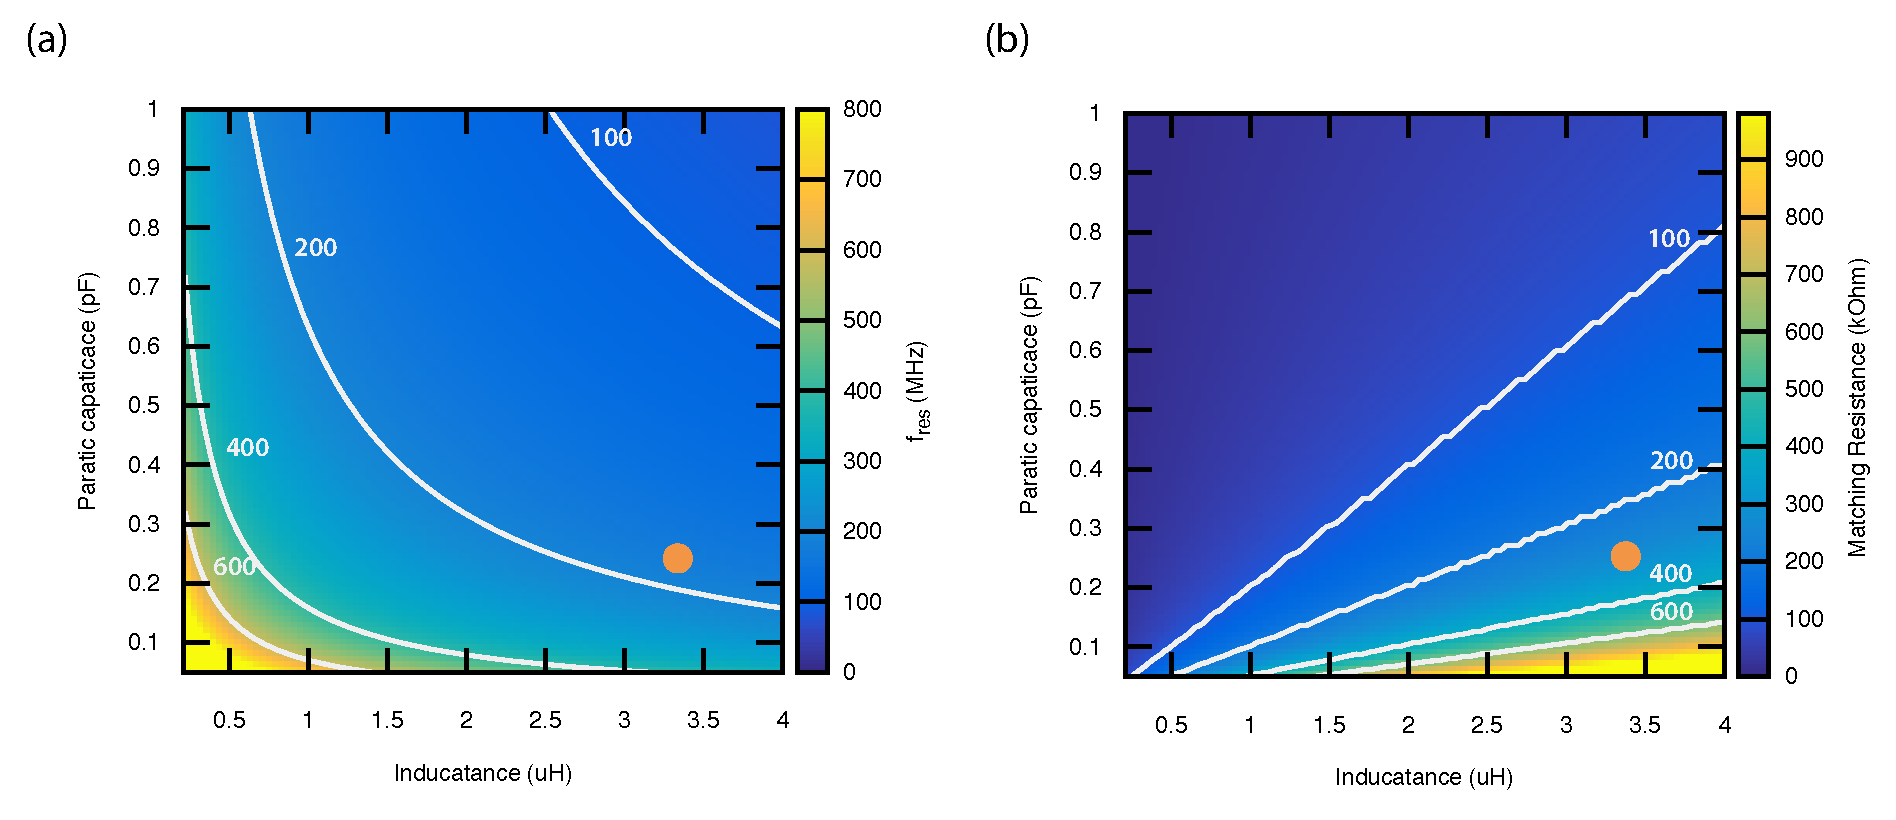
\includegraphics[width=\textwidth]{Illustrations/Theory_figure/theory_delft_v3.pdf}
		\caption{Circuit simulations for the circuit shown figure\ref{fig:overview}(c), where the inductance $L$ and the parasitic capacitance $C_p$ are varied. The resistance of the lead gate ($R_{lead}$) is set to $10M\Omega$ (typical value used in the experiment), the capacitance of the accumulation gate to the 2DEG is set to 1pF. The orange dot indicate the parameters for the device measured in this paper.}
		\label{fig:lead_gate_theory}
	\end{figure*}

	
	In this approach, the capacitance between the 2DEG and the accumulation gate is used as a feature rather than a bug.  The RF signal (RF in) is applied via the second accumulation gate as shown in figure \ref{fig:overview}(c).  The signal couples capacitively into the 2DEG ($C_{2DEG}$) and then travels to the sensing dot ($R_{sd}$). So compared to the Ohmic approach, this approach effectively swapped $R_{\rm 2DEG}$ and $C_{\rm 2DEG}$ in the model of Fig.\ \ref{fig:overview}(b), at high frequency $C_{\rm 2DEG}$ is a straight pass. A large capacitance of the accumulation gate is desirable as it causes a low impedance for the signal to travel into the 2DEG From simulations we estimated that a capacitance greater than 50fF (@200Mhz) is needed to not effect the matching condition of the circuit. In this case the circuit can effectively reduced to a RLC circuit.
	\\
	To ensure that the RF signal couples in via the accumulation gate and does not get effected by the lowly resistive ohmic, the lead gate (fig \ref{fig:overview}(c)) is introduced.
	Its function is to make a variable resistor ($R_{\rm lead}$) between the ohmic and the accumulation gate.
	When operated, its value is tuned $>>1M\Omega$ . We noticed that little difference is observed between operating the lead gate \textcolor{blue}{at $1M\Omega$ or open} \textcolor{red}{above 1 M$\Omega$}. This means it should possible to remove the ohmic all together, but this might make the tune up of the device harder, as no transport measurements are possible.
	\\
	To estimate the inductance is that needed to generate a good matching condition, we performed a simple simulation of the resonant circuit. As boundary conditions we require that the resonance frequency ($f_{res}$) that is greater than 100MHz (limited by the range of commercial amplifiers) and a matching resistance ($R_{MATCH}$) between $100k\Omega$ and $1M\Omega$ (typical resistance range for a sensing dot in SiGe).\\
	In figure \ref{fig:lead_gate_theory}(a) and  \ref{fig:lead_gate_theory}(b) we plot the resonance frequency, matching resistance for a given amount of parasitic capacitance ($C_p$) and inductance ($L$).
	From the simulations, we see that there is a large parameter space where we fulfill the requirements set before. The most sensitive parameter is the matching resistance. The simulation indicates that one should to design a chip that has a parasitic capacitance lower than 400fF, if this requirement if fulfilled, one should be able to find an suitable inductor value that gives good RF readout performance.\\
	In our case, the parasitic capacitance was around 250fF, where approximately 100fF originates from the bondwire and the remaining 150fF from the capacitance of the accumulation gate to the groundplane of the pcb. We used a superconducting high kinetic inductance inductor of 3.4uH to minimize self-capacitance of the inductor itself. The final matching resistance in our case is $275k\Omega$.  \color{red}do you have a rough idea of the PCB capacitor? \color{blue} $\rightarrow$ we don't use ground planes here + high kinetic inductance (=small footprint) inductors, so negligible compared to the rest of $C_p$.\color{black}
% subsection lead_gate_approach (end)

\section{Results} % (fold)
\label{sec:results}
\subsection{Ohmic Style RF Reflectometry with modified on board elements} % (fold)
	\label{sub:ohmic_style_rf_reflectometry_with_modified_on_board_elements}



\begin{figure}
	\includegraphics[width = \columnwidth]{Illustrations/HarvardFigure3_v5.pdf}
	\caption{Test the theory in figure\ \ref{fig:HarvardTheory} by changing the on board element then compare to the simulation.			
	(a-c) The reflection power as a function of $1/R_S$ of the same device with different lumped element capacitors and inductors as labeled. 		
	(d) The reflection power as a function of sensor gate voltage with fulled accumulated switch gate (left, minimum $R_{\rm cont}$) and partially accumulated switch gate (right, larger $R_{\rm cont}$) on the lead accumulation path. Center pannel: the current through the dot as a function of SD gate voltage at different $R_{\rm cont}$.}
	\label{fig:Harvardresult}
\end{figure}



	Ohmic style RF reflectometry has been demonstrated in GaAs but the additional capacitances introduced by the accumulation gates have made reproducing this in SiGe challenging.  We have identified four key strategies for device and circuit design that enable RF reflectometry in this system: blocking resistors ($R_{\rm block}$), capacitance management on the PCB ($C_0$), inductance tuning ($L$), and capacitance management on chip $C_{\rm gate}$.  
	
	We first focus on the PCB board modification so that it is compatible with the accumulation mode devices that are used in SiGe. As mentioned in the method part, we experimentally find a limit of improvement once $R_{\rm block}>10$ k$\Omega$ and thus we chose the this limit to compensate the blocking RF leakage and DC gate speed. With this optimized board we first experimentally verify the tunability of the tank circuit performance on $C_0$ and L. In figures 4a-c we show three different pairs of values with the same device and demonstrate that the  $R^{\rm match}_S$ can be altered dramatically. We begin with the C0 and L as suggested in Figure\ \ref{fig:HarvardTheory} (a-b). In (a) we have added a lumped element capacitance of 0.8 pF (total C0 of approximately 1.6 pF when the board capacitance of .8 pF is included) and $L = 2.7$ uH.  Even though the simulation indicates this value is far from boundary, the actual matching condition requires significantly lower conductance than what we can measure. A frequency shift is also observed at different $R_S$. This indicates a larger $C^*_{\rm gate}$ than what is expected in Figure\ \ref{fig:HarvardTheory} (a-b). In panel (b) we increase the lumped element capacitance to 2.2 pF (C0 = 2.2 pf+.8 pF=3 pF) with the same inductor as in (a). The frequency shift is gone with doubled C0, which means now the \{$C_0, L$\} set is far from the boundary. 
	However, the matching condition of  $R^{\rm match}_S = 50$ kOhm is too conductive for a quantum dot. An ideal matching condition is shown in Figure\ \ref{fig:Harvardresult}(c) with further increased inductor. In the end we achieve a best matching with an inductor of 6.8 uH giving a matching condition of 200 kOhm when the resonant frequency is around 34 MHz. By comparing these matching conditions we find a best fit with $R_{\rm cont}$ = 4 kOhm and $C^*_{\rm gate}$ = .45 pF. This may be over fit since as these device parameters may vary between cool downs. %and the same board components may change in their parameters when we hot soldering lumped elements.
	
	While we are able to drastically tune our matching conditions by using alternate tank circuit lumped elements, we find that the frequencies that we could achieve with this device design were lower than ideal as integration times will be longer for lower frequencies and RF components are less available. The final approach to improving tank circuit performance was improving the design of the quantum dot devices themselves.  
	
	By narrowing the lead accumulation gates by half before the gate approaches the sensor, we were able to reduce $C_{\rm gate}$ without increasing $R_{\rm cont}$ significantly.  This enabled the use of a significantly smaller $C_0$. We used only the board capacitance of $C_0 = 0.8$ pF and $L$ as low as 680 nH to achieve $R_S\sim 200$ kOhm and $f\sim 200$ MHz, which can be achieved with commercial cryogenic RF components. 	
	However, the tank circuit performance is very sensitive to the device. Any change in $R_{\rm cont}$, which is more dependent on the 2DEG mobility, or different $C_{\rm gate}$ that is dependent on the cap thickness would require different on-board elements to maintain a proper order of magnitude of $R^{\rm match}_s$ even for the same design. To further study the impact of $R_{\rm cont}$ and reduce the device dependence, we split the lead accumulate gate into two gates. One gate serves as ‘switch’ that turns on and off the connection from the Ohmic to the 2DEG and a channel that opens the electron path all the way to the sensor dot.
	
	In figure\ \ref{fig:Harvardresult}(d) we demonstrate a tuneable best matching $R_s$ around 50$\sim~$200 kOhm at a resonant frequency of 220 MHz. The outside two pannels plots the reflection power as a function of sensor dot gate voltage $V_{\rm PSL}$ at a higher (left panel) and lower (right panel) switch gate voltages. The middle panel plots corresponding the conductance of the sensor dot. With different gate voltage on the ‘switch’ gate, the total conductance through the dot is unchanged with the same voltages of all other gates, indicating a small back-action to the sensor tuning. In the contrast, the best matching is achieved with 1.5 nA for the fully accumulated switch gate, and 0.5 nA for a partial accumulated switch gate. The only difference between them is $R_{\rm cont}$ and this result agrees with the simulation in figure\ \ref{fig:Harvardresult} (c). This tunability allows the use of fixed $C_0$ and L for general devices as the matching condifion of the device can be changed in situ.
	
	The tunable $R_{\rm cont}$, however, is not the final solution because the larger $R_{\rm cont}$, more energy is lost before the sensor dot, resulting in a smaller signal. The parameter range of $C_0$ and $L$ is still narrow for this tuning scheme to work. For a device insensitive tank circuit with enough signal to noise, we need to further reduce the $C_{\rm gate}$ and $R_{\rm cont}$. One way to achieve that is to bring the Ohmic close to the dots, which reduce the metal area and shorten the distance of the lead 2DEG \cite{Connors2020}. Another is the lead gate approach.

% subsection ohmic_style_rf_reflectometry_with_modified_on_board_elements (end)

\subsection{Lead Gate Style RF Reflectometry} % (fold)
\label{sub:capacitive_style_rf_reflectometry}


\begin{figure}
	\includegraphics[width = \columnwidth]{Illustrations/Performance_figure/performance.eps}
	\caption{Characteristics and performance of the lead gate approach. In panel (a), the response of the matching circuit to a change in resistance of the sensing dot is shown. 
		Panel (b) shows the response of the resonant circuit at the resonance frequency versus the resistance of the sensing dot. The circuit matches at 275kOhm.
		Panel (c) shows a charge stability diagram of dot 3 and 4, measured via rf readout (2us per point). The black line in the figure shows the transition that is probed in panel (d).
		Panel (d) shows the infidelity of the charge detection versus measurement time. The green line shows the fidelity when going from the top to the bottom of a Coulomb peak of the sensing dot. The blue line shows the fidelity for detecting a dot-reservoir transition. The infidelity of the charge readout was estimated by sending a block pulse to the sensing dot or the quantum dot. When changing the frequency, one can check if it is possible to still differentiate the two signals generated by the block pulse (top and bottom of the pulse). The fidelity is estimated by making a histogram of both signal and calculating the overlap (similar to how one would do it for qubit readout).
	}
	\label{fig:lead_gate_result}
\end{figure}	


In figure \ref{fig:lead_gate_result}(a), the response of the resonator is shown for several resistances (below and above the matching point). From this figure one can derive the bandwidth of the matching circuit. At matching point, the expected bandwidth is 0.8MHz, in other words the minimal measurement time is 600ns (assuming a perfect SNR).
\\ \\
In panel (b) of figure \ref{fig:lead_gate_result} we characterized the reflectance of the matching circuit versus the resistance of the sensing dot. The matching point is $275k\Omega$. One can see that there are two highly sensitive regions around the matching point, one at $\sim200k$ and one at $\sim400k$. Note that that these regions do not overlap in the IQ plane as the phase flips 180$^\circ$ at $R_{match}$\footnote{measurement that shows this needs to be added.}.
The resistance of our sensing to was in the range of $400k\Omega$ to $1M\Omega$
, we speculate that it would be possible to further increase the SNR of the circuit by decreasing the parasitic capacitance ($C_p$) of $250fF$ to $150fF$ (e.g. by making the footprint of the gates smaller) to match to $600k\Omega$. \color{red} overall, are you looking into the in phase or quadrature of the reflected signal? The impedance matching is usually changes in the total power (in phase signal) instead of phase change (quadrature). Then emphasizing on the phase flip seems has nothing to do with what you are detecting? Or you just want to emphasis the location of the matching would be more reliable if you look into the phase? \color{blue} if a phase plot is made of the signal, lets say frequency vs Resistance of the SD, you would see that there is 180 degree flip when you go over the $f_{res}$, but the same also happens at the matching point $R_{Match}$. We measure along one axis in the IQ plane, as it contains all data. \color{black} 
\\ \\
Figure \ref{fig:lead_gate_result} (c-d) shows the performance one can expect from using this method. In (c) a charge stability diagram is shown. The acquisition time per point is set to 2us. This means that this readout is quite suitable for video mode tuning with high resolution ($>100\times100px$). In figure (d) we show the performance of the charge readout. There are two transitions probed. One is going from the top to the bottom of the coulomb peak of the sensing dot. From this measurement we should not be limited by the SNR and be able to measure the bandwidth of our system. We see that the charge readout fidelity strongly increases when measuring features equal or longer than 600-800ns. This matches with the bandwidth we extracted previously. To probe practical readout performance, we measured the charge fidelity of a dot reservoir transition. In this case the readout is not bandwith, but SNR limited. For this particular transition (see fig \ref{fig:lead_gate_result}(c)), we expect 99.9\% charge fidelity of the readout in 2us.

\section{Conclusion}
 
\printbibliography
	
% subsection capacitive_style_rf_reflectometry (end)
% section results (end)
\end{document}